%% TeX file for the TransportationTableaux user guide.
%% Code Author: Russell Andrew Edson, russell.andrew.edson@gmail.com

% Document setup parameters
\documentclass[a4paper,12pt]{article}
\topmargin -1cm
%\oddsidemargin -0.74cm
%\evensidemargin -0.74cm
%\textwidth 17.59cm
\textheight 23.94cm
\hyphenpenalty=100000
\parindent=0cm

% Import Libraries
\usepackage{amssymb}
\usepackage{amsmath}
\usepackage{amsfonts}
\usepackage{graphicx}
\usepackage{wrapfig}
\usepackage{caption}
\usepackage{bbding}
\usepackage[usenames,dvipsnames]{xcolor}
\usepackage{subcaption}
\usepackage{DejaVuSansMono}
\usepackage[cc]{titlepic}
\usepackage[titletoc,toc]{appendix}

\begin{document}

\Huge\textbf{TransportationTableaux User Guide} \\ \hspace*{1cm} \hrulefill \\
\normalsize

Created by Russell Andrew Edson \\
\texttt{russell.andrew.edson@gmail.com}\\
\texttt{https://github.com/RussellAndrewEdson/}\\

% Picture here.
\begin{figure}[h!]
\centering
\fbox{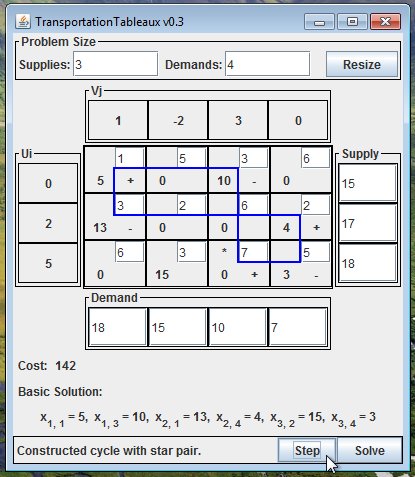
\includegraphics[width=0.8\textwidth]{transportationtableaux_v3screenshot.png}}
\end{figure}

\section*{TransportationTableaux}

The TransportationTableaux program was designed to solve Transportation problems in a step-by-step manner. Every detail of the solution process can be examined (the $u_i$/$v_j$ variables, finding the star pair, constructing the tableau cycle, adjusting the allocations, etc).\\

The main hope is that the program provides the user with a deeper understanding of how the solution process works. As such, it has primarily been developed as a teaching/demonstration tool.\\

\newpage

\section*{An example of a Transportation Problem}
Suppose we are given the following transportation problem to solve:\\

We have a situation where we have a group of suppliers that can satisfy demand for a particular commodity. (This can be anything; for the sake of the example, suppose that we have a group of paper suppliers that can deliver paper to places that need it.)\\

Now each supplier will have a different amount of paper that they can supply:
\begin{itemize}
\item
Supplier $S_A$ has 15 tons of paper available.
\item
Supplier $S_B$ has 17 tons of paper available.

\item
Supplier $S_C$ has 18 tons of paper available.\\
\end{itemize}

Just as the suppliers will have different amounts that they can supply, their customers will have different levels of demand:
\begin{itemize}
\item
Customer $D_A$ demands 18 tons of paper. 

\item
Customer $D_B$ demands 15 tons of paper.

\item
Customer $D_C$ demands 10 tons of paper.

\item
Customer $D_D$ demands \;\;7 tons of paper.

\end{itemize}

Note that the total supply equals the total demand (we call such a problem a \textit{Balanced Transportation Problem}). This crucial fact is what allows our algorithm to work, but you can always balance an unbalanced problem (just add fictitious suppliers or customers to pick up the slack.) \\

Of course, there's always a cost associated with moving stuff from one place to another; eg. it might cost 1-hundred dollars to transport a single ton of paper from supplier $S_A$ to customer $D_A$, but 5-hundred dollars to transport a ton of paper from supplier $S_A$ to customer $D_B$. So it is 5 times more expensive for Supplier $S_A$ to send paper to customer $D_B$. (The actual cost is not so important, just the relative magnitudes between the costs.)\\

We represent this with the \textit{link-flow cost matrix}:\\

\begin{tabular}{| l | r | r | r | r | }
\hline
From/To & Customer $D_A $ & Customer $D_B $ & Customer $D_C $ & Customer $D_D $ \\
\hline
Supplier $S_A$ & 1 & 5 & 3 & 6 \\
\hline
Supplier $S_B$ & 3 & 2 & 6 & 2 \\
\hline 
Supplier $S_C$ & 6 & 3 & 7 & 5  \\
\hline
\end{tabular}\\[6pt]

(* If we had fictitious suppliers and customers, they would have a transport cost of 0 to everything else in this matrix.)\\

\newpage

So we wish to find the \textbf{smallest possible cost of transportation}: that is, we wish to meet all demand, but in the cheapest way possible.\\

We do this using the \textit{Primal-Dual Transportation Algorithm}. The explanation of the algorithm involves some complex mathematics and is (for the moment) beyond the scope of this guide. But we don't have to worry about it -- the program takes care of the entire solution process.\\

(For those that already have some knowledge of the algorithm: as you'll see, the program displays all of the information from its solution process, so you can see exactly how the algorithm works anyway.)\\

\section*{Solving with the TransportationTableaux program}
So given the above example, all we need to do is enter the values into the fields of the program.

\begin{enumerate}
\item
Upon first firing up the program, the default tableau size is for a problem with 3 supplies and 3 customers (demands).

\begin{figure}[h!]
\centering
\fbox{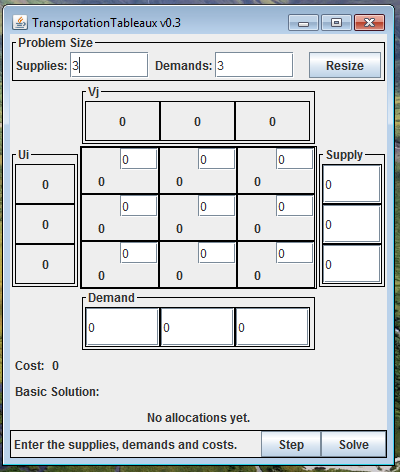
\includegraphics[width=0.72\textwidth]{screen01.png}}
\caption{The initial tableau for the program after startup.}
\end{figure}

\newpage

\item
However, we have a problem with 4 demands, so we adjust the number of demands and hit 'Resize'.

\begin{figure}[h!]
\centering
\fbox{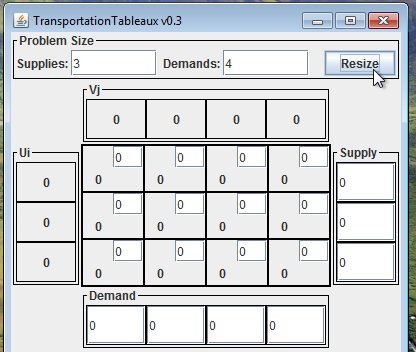
\includegraphics[width=0.75\textwidth]{screen02.png}}
\caption{We can resize the tableau by clicking the 'Resize' button.}
\end{figure}

\item
We then enter in the values for the supplies into the fields as shown. (ie. the number of tons of paper available to each supplier, in the case of our example.) We've entered them in the order $S_A$, $S_B$, $S_C$ here, but note that the order is arbitrary at this point.

\begin{figure}[h!]
\centering
\fbox{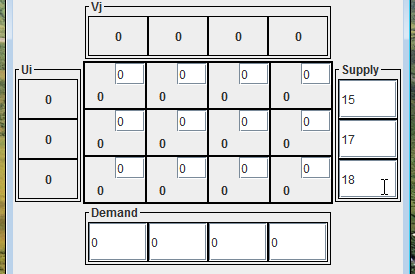
\includegraphics[width=0.75\textwidth]{screen03.png}}
\caption{The values for the supplies can be entered straight into the grid.}
\end{figure}

\newpage

\item
Similarly, we enter in the values for the demands (customers). The order is still arbitrary at this point, but for simplicity we've simply entered them in the order $D_A$, $D_B$, $D_C$, $D_D$ as we go from left to right.

\begin{figure}[h!]
\centering
\fbox{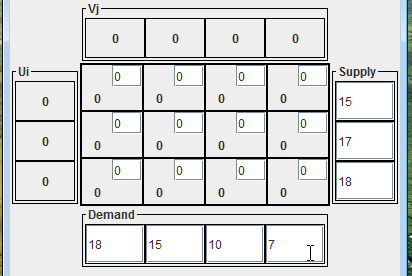
\includegraphics[width=0.75\textwidth]{screen04.png}}
\caption{The values for the demands can also be entered straight into the grid.}
\end{figure}

\item
Next, we enter in the link-flow costs. However, now the order does matter -- we line up each supply and demand with its corresponding transportation cost. (So the first supply box is $S_A$ and the first demand box is $D_A$, so the box in row 1, column 1 of the grid is the cost of transporting from $S_A$ to $D_A$, and so on.) 

\begin{figure}[h!]
\centering
\fbox{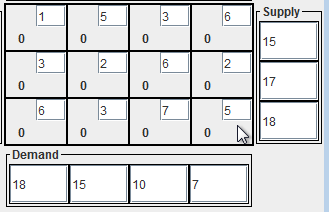
\includegraphics[width=0.75\textwidth]{screen05.png}}
\caption{Each link-flow cost can be entered into the top-right corner of the grid cells.}
\end{figure}

\newpage

\item
We can now simply step through the solution to the problem (or if you're in a hurry, simply press 'Solve' to jump straight to the optimal solution tableau.)

\begin{figure}[h!]
\centering
\fbox{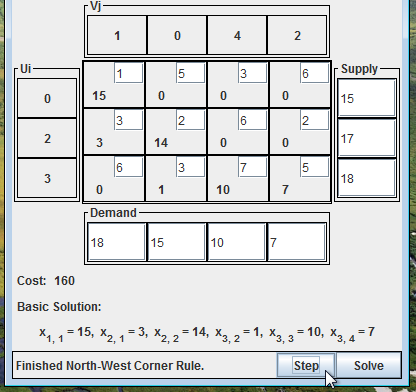
\includegraphics[width=0.75\textwidth]{screen06.png}}
\caption{Once the values have been entered, press 'Step' to begin the solution process with the North-West corner rule.}
\end{figure}

The North-West corner rule is performed to give us an initial solution to the problem, but it probably won't be optimal. The cost and basic solution are shown below the tableau (the basic solution should be read as: $x_{1,1} = 15$ means that the 1st supply $S_A$ should send 15 tons of paper to the 1st demand $D_A$. )\\ 

For those with knowledge of the Primal-Dual Transportation algorithm, note that the $u_i$ and $v_j$ dual variables have also been found for the new tableau. These appear in the outer row and columns as shown. \\

\newpage

\item
Now the solution found by the North-West corner rule is not optimal. So we aim to modify our allocations toward a more optimal solution, and we do this in a methodical way by making sure that our adjustments always give us a smaller cost (by seeking \textit{dual feasibility}, a concept that is out of the scope of this tutorial).\\

Suffice it to say that we (methodically) find a supply-demand pair that doesn't already have an allocation, and give it one. We call such a pair a \textit{star-pair}. Clicking 'Step' again will have the program find this pair for us.\\

 \begin{figure}[h!]
\centering
\fbox{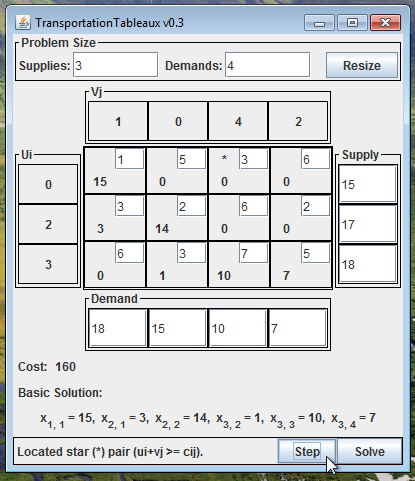
\includegraphics[width=0.75\textwidth]{screen07.png}}
\caption{Pressing 'Step' again finds us the star-pair.}
\end{figure} 

The star-pair can be seen in the grid, marked with a $*$ in the top-left corner.\\

\newpage

\item
Of course, keep in mind that our transportation problem is balanced, and our initial solution from the North-West corner rule already allocated all of the supply. So if we want to give the star-pair an allocation, we need to make adjustments to all of the other supply-demand pairs too!\\

To explain this, suppose we wish to give the star-pair (at row 1, column 3) an allocation of 2. Then to keep the supply balanced, we need to remove a total of 2 from the other allocations in the same row (row 1); and to keep the demand balanced, we need to remove a total of 2 from the allocations in the same column (column 3).\\

But then since we removed 2 from the supply-demand pair at row 1, column 1, this has thrown the demand in column 1 out of balance. So we need to add 2 back to some other allocation in column 1, which will further throw the tableau out of balance if we're not careful about it. Things get pretty dicey very quickly!\\

We handle this by finding a cycle in the tableau through the star-pair and the existing allocations. The program will do this for us when we click 'Step' again.

\begin{figure}[h!]
\centering
\fbox{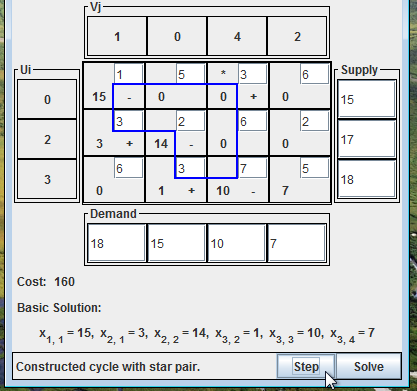
\includegraphics[width=0.75\textwidth]{screen08.png}}
\caption{Clicking 'Step' will now give us our cycle along which to adjust the allocations safely.}
\end{figure} 

\newpage

Note also that in addition to the cycle, some $+$ and $-$ signs have shown up in the bottom-right corner of those cells at the vertices of the cycle.

\begin{figure}[h!]
\centering
\fbox{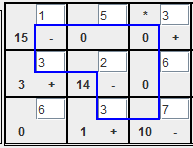
\includegraphics[width=0.37\textwidth]{screen081.png}}
\caption{The tableau cycle.}
\end{figure} 

In terms of the adjustments, the $+$ signifies that the allocation for that supply-demand pair will be increased for the next tableau. Likewise, the $-$ signifies that the allocation will be decreased.\\

The star-pair always has its allocation increased (that was the whole point, remember?) and we alternate $+$, $-$, $+$, $-$ as we walk along the cycle. This fixes our allocation problem mentioned earlier; every time we increase ($+$) an allocation, we also decrease ($-$) another allocation from the same row and the same column, and vice versa. So everything balances out.\\

As for the amount that the allocations are adjusted by? This is chosen to be the minimum of all of the current allocations that are to be decreased ($-$). The reasoning is beyond the scope of this tutorial, but choosing this amount works.\\

\newpage

\item
Finally, clicking 'Step' again will adjust the allocations along the cycle and bring us to the next tableau.

\begin{figure}[h!]
\centering
\fbox{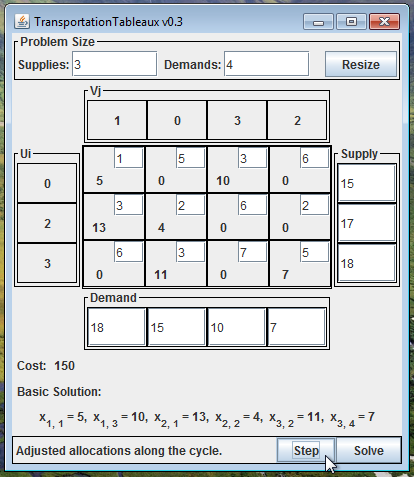
\includegraphics[width=0.75\textwidth]{screen09.png}}
\caption{Clicking 'Step' adjusts the allocations in the grid.}
\end{figure}

Note that the cost has decreased (as we'd hoped), and the basic solution has changed. (The $u_i$ and $v_j$ variables have also been recalculated for the new tableau.)\\

The tableau is still not optimal yet though. So we repeat the process -- we find the star-pair, construct the cycle, and adjust the allocations along the cycle accordingly to get to the next tableau, which will have a more optimal solution. Clicking 'Step' repeatedly will take us through each of these steps in turn, showing the star-pairs, cycles and tableau at every stage.\\

(Note that sometimes the cost might not have changed. This happens when the adjustment does not modify the total cost of transportation, but simply changes the supply-demand pairs around so that it can get to a smaller cost later.)\\

\newpage

\item
Finally, when you've arrived at the last tableau (or when you've skipped right to the end by clicking the 'Solve' button), you'll be told such in the status at the bottom of the window. (The buttons will also be disabled, as shown.)

\begin{figure}[h!]
\centering
\fbox{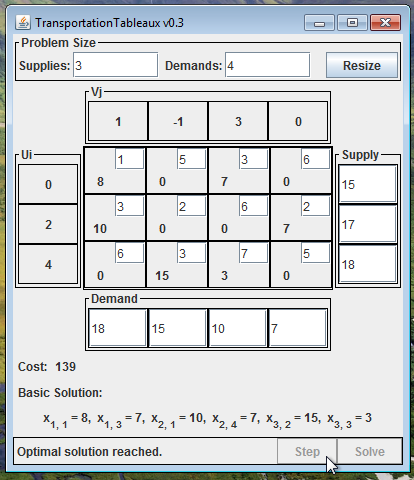
\includegraphics[width=0.75\textwidth]{screen10.png}}
\caption{We've reached the last tableau with the optimal solution.}
\end{figure}

The cost given here is the minimum possible cost of transportation for the problem that results in all of the demand being met.The basic solution gives the allocations for this minimum cost.\\

So we've solved the problem! The minimum cost for our example is\\ 139(-hundred dollars), achieved when we send:
\begin{itemize}
\item 8 \;\;tons of paper from supplier $S_A$ to customer $D_A$,
\item 7 \;\;tons of paper from supplier $S_A$ to customer $D_C$,
\item 10 tons of paper from supplier $S_B$ to customer $D_A$,
\item 7 \;\;tons of paper from supplier $S_B$ to customer $D_D$,
\item 15 tons of paper from supplier $S_C$ to customer $D_B$,
\item 3 \;\;tons of paper from supplier $S_C$ to customer $D_C$.
\end{itemize}

\end{enumerate}


\end{document}
